
\documentclass[aspectratio=169]{beamer}

%\setbeameroption{hide notes}
%\setbeameroption{show notes}
%\setbeameroption{show only notes}

  % Copyright (C) 2012 - EDF R&D - Michael Baudin

% To highlight source code
\usepackage{listings}
\definecolor{darkgreen}{rgb}{0,0.5,0}
\definecolor{violet}{rgb}{0.5,0,1}

\usepackage{lmodern}% http://ctan.org/pkg/lm

\usetheme{Montpellier}
\setbeamertemplate{navigation symbols}{} % Remove navigation
\useoutertheme{infolines}

\usepackage[utf8]{inputenc}
\usepackage[T1]{fontenc}

%\usepackage[french]{babel}
%\uselanguage{French}
%\languagepath{French}

\def\bx{{\bf x}}
\def\RR{\mathbb{R}}

\newcommand{\pyvar}[1]{\texttt{#1}}

\def \ot {OpenTURNS}

\hypersetup{colorlinks=true}

\usepackage{adjustbox}
\usepackage[normalem]{ulem}

\title[OpenTURNS]{OpenTURNS release highlights}

\author[OpenTURNS et al.]{J. Schueller (Phimeca)}

% \institute[Airbus-EDF-IMACS-ONERA-Phimeca]{
% \inst{1} Airbus
% \inst{2} EDF R\&D. 6, quai Watier, 78401, Chatou Cedex - France, michael.baudin@edf.fr \and %
% \inst{3} IMACS
% \inst{4} ONERA
% \inst{5} Phimeca Engineering. 18/20 boulevard de Reuilly, 75012 Paris - France, schueller@phimeca.com
% }

\date[]{User Day \#16, June 23rd 2023, EDF Lab}
%%%%%%%%%%%%%%%%%%%%%%%%%%%%%%%%%%%%%%%%%%%%%%%%%%%%%%%%%%%%%%%%%%%%%%%%%%%%%

  \begin{document}

%%%%%%%%%%%%%%%%%%%%%%%%%%%%%%%%%%%%%%%%%%%%%%%%%%%%%%%%%%%%%%%%%%%%%%%%%%%%%

  \begin{frame}
  \titlepage

  \begin{columns}
  \begin{column}[t]{0.05\textwidth}
        \end{column}
  
    \column{0.10\textwidth}
  \begin{center}

\includegraphics[height=0.04\textheight]{figures/airbus-logo-3d-blue.png}
\end{center}

    \column{0.05\textwidth}
  \begin{center}

\includegraphics[height=0.09\textheight]{figures/logo-edf.jpg}
\end{center}

     \column{0.05\textwidth}
  \begin{center}

\includegraphics[height=0.09\textheight]{figures/imacs-logo.jpg}
\end{center}

    \column{0.10\textwidth}
  \begin{center}

\includegraphics[height=0.05\textheight]{figures/onera-logo.png}
\end{center}

    \column{0.15\textwidth}
  \begin{center}

\includegraphics[height=0.08\textheight]{figures/logo-phimeca.png}
\end{center}

\column{0.01\textwidth}

  \end{columns}

  \end{frame}

\begin{frame}
\frametitle{Overview}

New features since last year in releases:

\begin{itemize}
\item v1.20: fall 2022
\item v1.21: \sout{spring} summer 2023
\end{itemize}

\end{frame}
  
%%%%%%%%%%%%%%%%%%%%%%%%%%%%%%%%%%%%%%%%%%%%%%%%%%%%%%%%%%%%%%%%%%%%%%%%%%%%%

% \begin{frame}
% \frametitle{Contents}
% % \tableofcontents
% \end{frame}

%%%%%%%%%%%%%%%%%%%%%%%%%%%%%%%%%%%%%%%%%%%%%%%%%%%%%%%%%%%%%%%%%%%%%%%%%%%%%

\begin{frame}{Smolyak quadratures}

\begin{itemize}
\item Combination of tensorized quadratures to build an n-d DOE from n 1-d DOEs
\item The combination technique reduces the nodes number wrt raw tensorization rule
\item Fine-grained control over the nodes/weights merging step, access m-indices
\item Designed to be used for functional chaos (by integration or least-squares)
\end{itemize}

\begin{figure}[!htb]
\minipage{0.5\textwidth}
  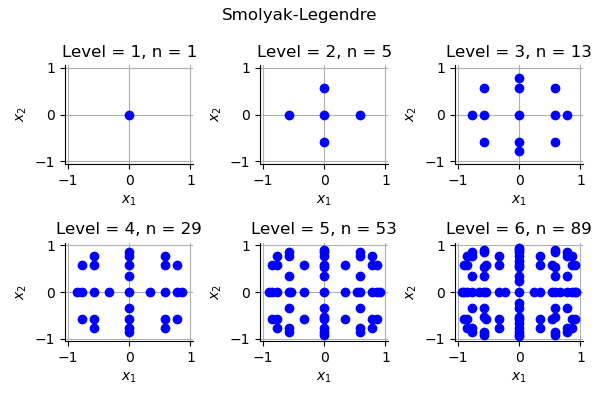
\includegraphics[width=0.9\textwidth]{figures/smolyakplot}
\endminipage\hfill
\minipage{0.5\textwidth}
  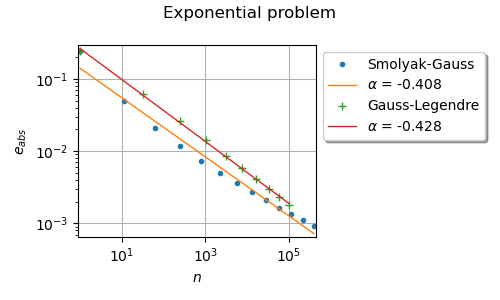
\includegraphics[width=0.9\textwidth]{figures/sphx_glr_plot_smolyak_quadrature_001}
\endminipage
\end{figure}
\end{frame}

%%%%%%%%%%%%%%%%%%%%%%%%%%%%%%%%%%%%%%%%%%%%%%%%%%%%%%%%%%%%%%%%%%%%%%%%%%%%%

\begin{frame}{Cross-entropy importance sampling 1/2}

\begin{itemize}
\item Adaptive, importance-sampling based simulation algorithm

\item Update an intermediate threshold $q_k$ at each step

$$\rho \in [0,1], q_k=\max(T,y^{(k)}_{\left \lfloor \rho N \right\rfloor})$$

\item Auxiliary distribution $h$ parameters $\underline{\lambda}$ numerically optimized at each step
% $$$$
$$\underline{\lambda}_{k}= \textrm{argmax}_{\lambda} \frac{1}{N} \sum_{i=1}^{N}{\underline{1}}_{g(\underline{x}_i^{(k)}) \leq q_k} \frac{f_\underline{X}(\underline{x}_i^{(k)})}{h_{\underline{\lambda}_{k-1}}(\underline{x}_i^{(k)})} \log(h_{\underline{\lambda}}(\underline{x}_i^{(k)}))$$

\item Compute the final importance probability

$$\widehat{P}^{CE}(g(\underline{\underline{X}})<T)=\frac{1}{N}\displaystyle \sum_{i=1}^{N} \underline{1}_{g(\underline{x}_i^{(k)})<T} \frac{f_\underline{X}(\underline{x}_i^{(k)})}{h_{\underline{\lambda}_{k-1}(\underline{x}_i^{(k)})}}$$

\end{itemize}
\end{frame}

\begin{frame}{Cross-entropy importance sampling 2/2}

\begin{itemize}
\item Standard space variant with analytical optimum of the Normal parameters
\item Very good performance, can be compared to subset
\item Also, no COV-based termination criterion (based on threshold)
\end{itemize}

\begin{figure}
   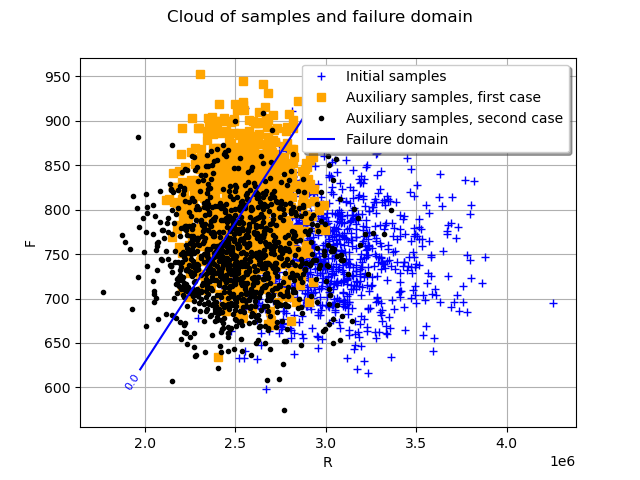
\includegraphics[width=0.5\textwidth]{figures/sphx_glr_plot_crossentropy_003}
   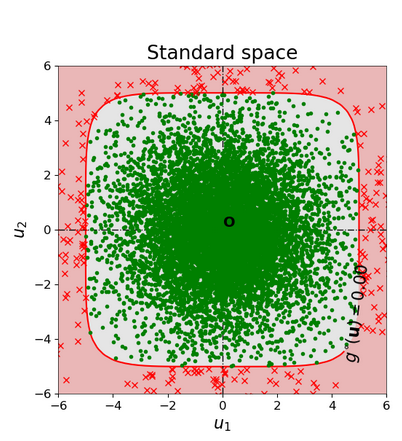
\includegraphics[width=0.35\textwidth]{figures/crossads}
\end{figure}

\end{frame}

%%%%%%%%%%%%%%%%%%%%%%%%%%%%%%%%%%%%%%%%%%%%%%%%%%%%%%%%%%%%%%%%%%%%%%%%%%%%%

% \section{Uniform distribution over a mesh}

\begin{frame}{Uniform distribution over a mesh}
% \begin{block}
\begin{itemize}
\item Uniform sampling in any closed set delimited by a generic mesh, any dimension
\item Sampling of simplices weighted by volume, then uniform sampling inside simplex
\item CDF is obtained by integration at mesh bounds
\item Efficient implementation, low-level primitives for tetras, etc ...
\end{itemize}
% \end{block}
\begin{figure}
   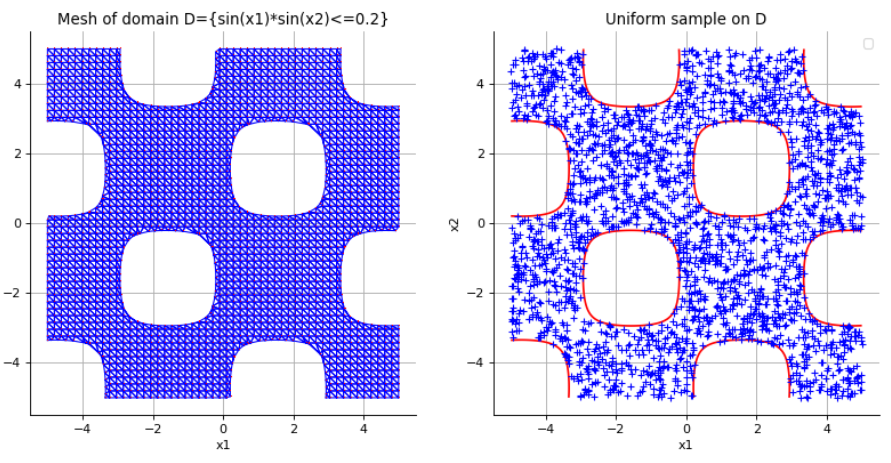
\includegraphics[width=0.6\textwidth]{figures/UniformOverMesh}
\end{figure}
\end{frame}

%%%%%%%%%%%%%%%%%%%%%%%%%%%%%%%%%%%%%%%%%%%%%%%%%%%%%%%%%%%%%%%%%%%%%%%%%%%%%

\begin{frame}
\frametitle{HSIC performance improvements}
\begin{itemize}
\item Loop reordering and parallelization of P-Values evaluation (permutation) using TBB
\item Efficient trace computation in HSICVStat instead of full products
\item Cache input covariance matrix discretization
\item Use STL primitives like std::accumulate
\end{itemize}

\vspace{6pt}

\begin{block}{Benchmark (global HSIC, 3 OT versions, 2 estimators, 2 sizes, 2 p-values types)}
\begin{tabular}{lllllll}
version/ustat|vstat & 1.19/U & 1.20/U & 1.21/U & 1.19/V & 1.20/V & 1.21/V \\
time (100/perm) & 1.30 & 1.31 & 0.082 & 6.65 & 6.70 & 0.01\\
time (1000/perm) & - & 762.8 & 36.58 & - & 5313.4 & 0.79\\
time (100/asymp) & 0.028 & 0.028 & 0.0013 & 0.028 & 0.031 & 0.0017\\
time (1000/asymp) & 16.59 & 16.46 & 0.17 & 16.56 & 17.85 & 0.15\\
\end{tabular}
\end{block}

\end{frame}

%%%%%%%%%%%%%%%%%%%%%%%%%%%%%%%%%%%%%%%%%%%%%%%%%%%%%%%%%%%%%%%%%%%%%%%%%%%%%

\begin{frame}
\frametitle{Chaos rewrite}
\begin{itemize}
\item Long-term effort to simplify usage and improve performance
\item Deduplicate basis selection at AdaptiveStrategy and LARS level
\item Restrict combination of integration + LARS
\item New LeastSquaresExpansion and IntegrationExpansion classes available in 1.21
\item Ongoing work to rewrite LARS selection as well (2024 ?)
\end{itemize}

% \vspace{6pt}
% 
% \begin{block}{Benchmark (Ishigami, basis size=455, sampling size=8192)}
% \begin{tabular}{lll}
% version & old & new \\
% time (integration) & &\\
% time (least-squares) & &\\
% \end{tabular}
% \end{block}

\begin{center}
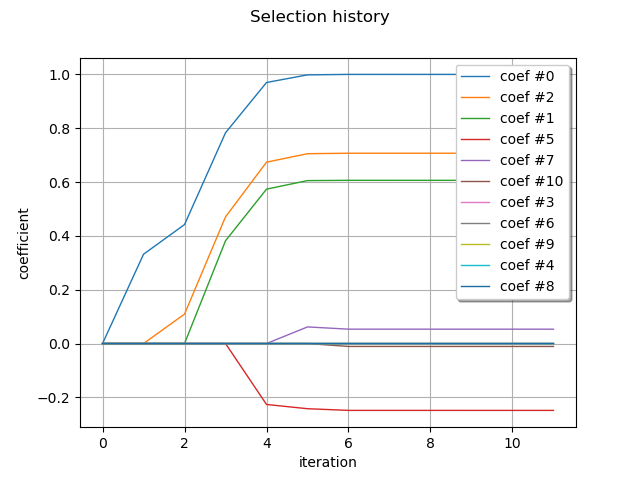
\includegraphics[width=0.4\textwidth]{figures/lars}
\end{center}

\end{frame}

%%%%%%%%%%%%%%%%%%%%%%%%%%%%%%%%%%%%%%%%%%%%%%%%%%%%%%%%%%%%%%%%%%%%%%%%%%%%%

\begin{frame}
\frametitle{Documentation improvements}
\begin{itemize}
\item Lots of new examples: chaos, cv, regression, MLE, functions, integration, enumerate, ...
\item New usecases: fire satellite, wing weight, Linthurst/Coles datasets
\end{itemize}

\begin{center}
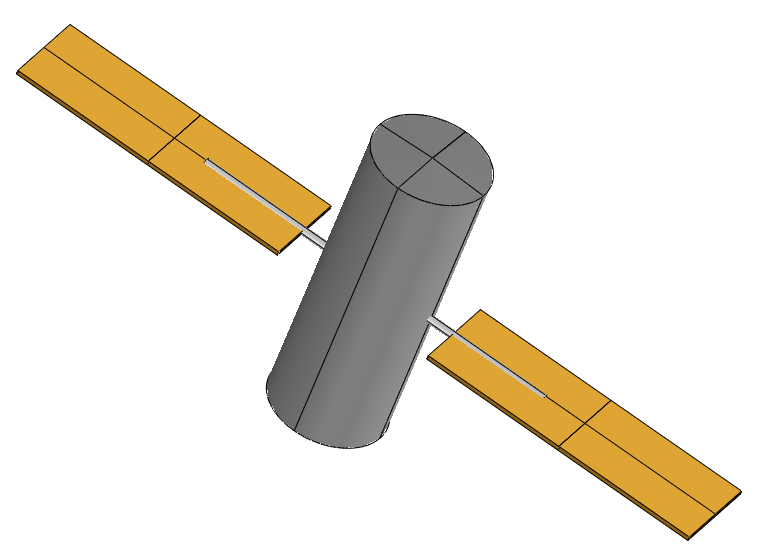
\includegraphics[width=0.3\textwidth]{figures/firesatellite}
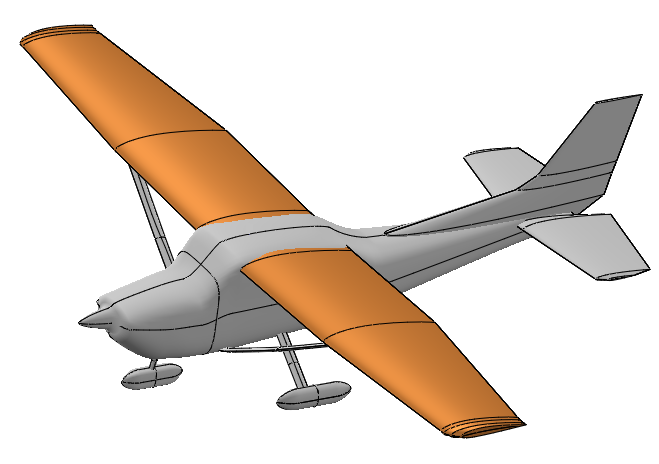
\includegraphics[width=0.3\textwidth]{figures/wingweight}
\end{center}

\begin{itemize}
\item Example minigalleries linking to relevant examples
\item Lot of time invested in the improvement of the documentation
\end{itemize}
\end{frame}

%%%%%%%%%%%%%%%%%%%%%%%%%%%%%%%%%%%%%%%%%%%%%%%%%%%%%%%%%%%%%%%%%%%%%%%%%%%%%

\begin{frame}
\frametitle{Other improvements}
\begin{itemize}
\item Improved MCMC adaptation and new class to customize the update
\item Field to vector metamodeling and sensitivity using KL + chaos
\item Chaos expansion for mixed variables
\item New BoxCoxFactory method to return directly the underlying linear model
\item New inference method based on quantile numerical optimization
\item Enabled Pagmo.moead\_gen, Bonmin.Ecp/iFP optimization algorithms
\item Continued bugfix effort (avg 30+ recorded per release + more internally fixed)
\end{itemize}

\vspace{6pt}

\begin{center}

\includegraphics[width=0.15\textwidth]{figures/bugfix}
\end{center}

\end{frame}

%%%%%%%%%%%%%%%%%%%%%%%%%%%%%%%%%%%%%%%%%%%%%%%%%%%%%%%%%%%%%%%%%%%%%%%%%%%

\begin{frame}
\frametitle{Packaging 1/2}
\begin{block}{Python channels}
\begin{itemize}
\item Pip, Conda
\item Versions: 3.8-3.11
\item OS: Windows, Linux, MacOS
\item Architectures: x86\_64, arm64 (MacOS-only)
\end{itemize}
\end{block}

\begin{figure}
   
\includegraphics[width=0.3\textwidth]{figures/PyPI_logo}
   
\includegraphics[width=0.3\textwidth]{figures/Conda_logo.svg}
\end{figure}

\end{frame}

\begin{frame}
\frametitle{Packaging 2/2}
\begin{block}{Supported Linux distributions}
\begin{itemize}
\item Ubuntu 20/22
\item Debian 11/12
\item Fedora 37/38
\item CentOS 8
\item OpenSUSE 15.4
\item Mageia 8
\item ArchLinux
\end{itemize}

... and FreeBSD

\end{block}


\begin{center}

\includegraphics[width=0.05\textwidth]{figures/debian-openlogo-100}

\includegraphics[width=0.08\textwidth]{figures/ubuntu}

\includegraphics[width=0.08\textwidth]{figures/Fedora-Logo}

\includegraphics[width=0.08\textwidth]{figures/centos-logo}

\includegraphics[width=0.08\textwidth]{figures/opensuse-logo}

\includegraphics[width=0.15\textwidth]{figures/200px-Logo_mageia_official}

\includegraphics[width=0.15\textwidth]{figures/archlinux-logo}

\includegraphics[width=0.15\textwidth]{figures/FREEBSD_Logo_Horiz_Pos_RGB}
\end{center}

\end{frame}

%%%%%%%%%%%%%%%%%%%%%%%%%%%%%%%%%%%%%%%%%%%%%%%%%%%%%%%%%%%%%%%%%%%%%%%%%%%%%

\begin{frame}
\frametitle{END}

Thank you for your attention!

Any questions?

\begin{center}
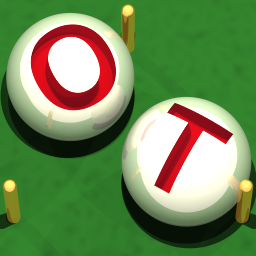
\includegraphics[width=0.2\textwidth]{figures/logo-ot-small}
\end{center}

\end{frame}

% %%%%%%%%%%%%%%%%%%%%%%%%%%%%%%%%%%%%%%%%%%%%%%%%%%%%%%%%%%%%%%%%%%%%%%%%%%%%%
% 
% \section{Bibliography}
% 
% \begin{frame}
% \frametitle{Bibliography}
% 
% \begin{itemize}
% \item Airbus, EDF, ONERA, Phimeca Engineering, IMACS.
% OpenTURNS, a scientific library usable as a Python module dedicated to the treatment of uncertainties, 
% \url{www.openturns.org}.
% \item Airbus, EDF, Phimeca Engineering, IMACS. Documentation of OpenTURNS, version 1.9. 
% \url{http://openturns.github.io/openturns/1.9/contents.html}
% \item  Michaël Baudin, Anne Dutfoy, Bertrand Iooss, and Anne-Laure Popelin. 
% OpenTURNS: An Industrial Software for Uncertainty Quantification in Simulation, 
% Handbook of Uncertainty Quantification, 
% pages 1-38. Springer International Publishing, 2016
% \end{itemize}
% 
% \end{frame}

\end{document}
